\section{个人简介}

\subsection{Education}

\begin{xframe}{Education}
    \cveducation
    {\entrylocationstyle{华中科技大学}}
    { }

    \vspace{2.0mm}

    \cvsubeducation
    {管理学院}
    {09/2015 - 03/2018}

    \vspace{-2.5mm}
    \begin{itemize}
        \item \descriptionstyle{会计硕士,主修, GPA 3.8/4.0\\
              {核心课程: 财务管理理论与实务, 管理会计理论与实务, 审计理论与实务,内部控制理论与实务,金融市场与金融工具}}

              \vspace{2.5mm}

        \item \descriptionstyle{计算机科学与技术,选修,GPA:3.6/4.0\\
              {核心课程: 高等工程数学(矩阵论 \& 数理统计 \& 数值计算), 人工智能, 模式识别, 知识发现与数据开采, 大数据技术}}
    \end{itemize}

    % \cvsubeducation
    % {计算机科学与技术学院}
    % {09/2016 - 02/2017}

    % \vspace{-2.5mm}
    % \begin{itemize}
    %     \item \descriptionstyle{计算机科学与技术,选修,GPA:3.6/4.0}
    %     \item \descriptionstyle{\itshape{核心课程: 高等工程数学(矩阵论 \& 数理统计 \& 数值计算), 人工智能, 模式识别, 知识发现与数据开采, 大数据技术, 启发式优化}}
    % \end{itemize}



\end{xframe}

\begin{xframe}{Education}
    \cveducation
    {\entrylocationstyle{中南财经政法大学}}
    { }

    \vspace{2.0mm}

    \cvsubeducation
    {会计学院}
    {09/2011 - 06/2015}

    \vspace{-2.5mm}

    \begin{itemize}
        \item \descriptionstyle{会计学学士\\
              {核心课程: 会计学原理,中级会计学,管理会计学(双语),企业资源计划,会计实验学,会计电算化}}
              % \item \descriptionstyle{\itshape{核心课程: 会计学原理,中级会计学,管理会计学(双语),企业资源计划,会计实验学,会计电算化}}
    \end{itemize}

\end{xframe}

\subsection{Research}

\begin{xframe}{Research}
    \cvexperience
    {\entrylocationstyle{研究助理},管理学院,蔡淑琴教授}
    {09/2015 - 08/2017}

    \vspace{-2.5mm}

    \begin{itemize}
        \item \descriptionstyle{结合句法结构与向量空间模型,提出一种考虑抱怨问题路径的网络抱怨识别方法;}
        \item \descriptionstyle{考虑知识、情感和互动三个资源维度,建立处理在线负面口碑的专家识别方法;}
        \item \descriptionstyle{基于会计核算视角,通过词嵌入与循环神经网络实现端到端的账务智能处理框架;}
    \end{itemize}

    \cvexperience
    {\entrylocationstyle{研究助理},管理学院,大数据实验室}
    {03/2016 - 08/2017}

    \vspace{-2.5mm}

    \begin{itemize}
        \item \descriptionstyle{实现基于ZigBee的区域定位接口与基于RFID的电子标签读写接口;}
        \item \descriptionstyle{搭建基于Hadoop的全分布式计算机集群,实现Map/Reduce框架下的Naïve Bayes分类器;}
    \end{itemize}

\end{xframe}

\begin{xframe}{Dissertation}
    \begin{itemize}
        \item \descriptionstyle{端到端的账务智能处理框架}
    \end{itemize}

    \vspace{1.0mm}

    
\includegraphics[width=\textwidth]{./style/images/accounting.png}
\end{xframe}

\begin{xframe}{Dissertation}
    \begin{itemize}
        \item \descriptionstyle{会计事项的机器理解:利用Word2Vec方法实现会计事项的词向量空间嵌入;}
    \end{itemize}


    \begin{columns}
        \column{0.4\textwidth}<1->
        \begin{center}
            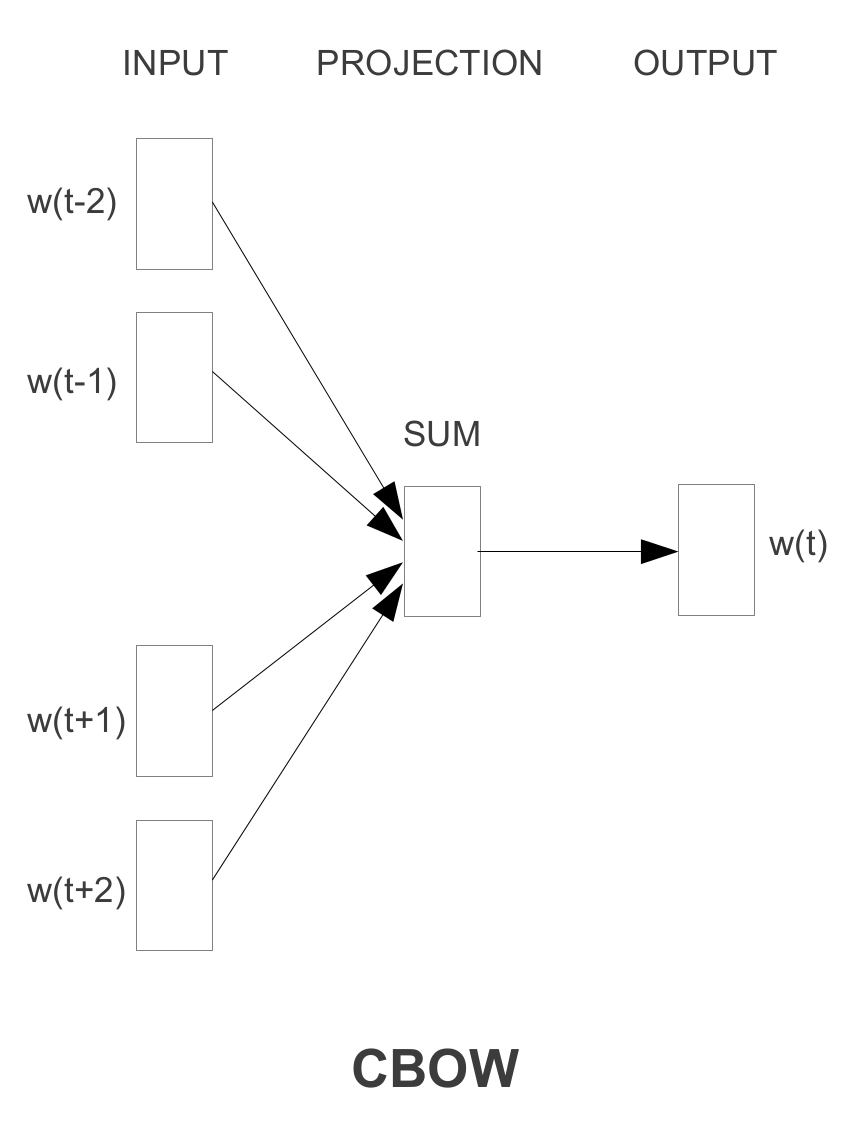
\includegraphics[height=0.7\textheight]{./style/images/w2v_net.png}
        \end{center}
        \column{0.6\textwidth}<1->
        \begin{center}
            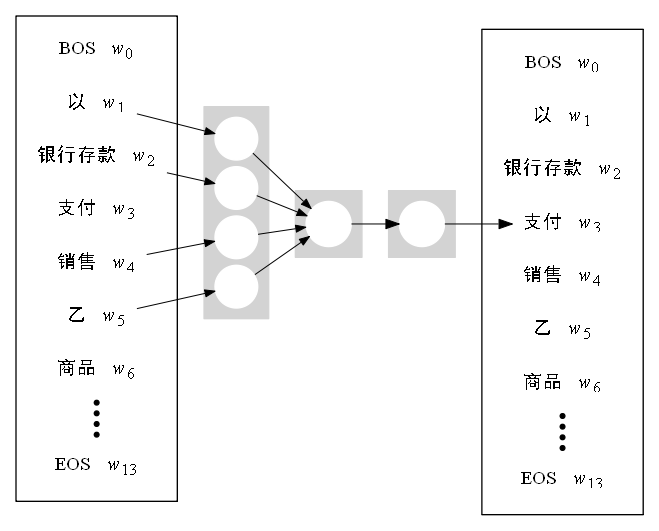
\includegraphics[height=0.6\textheight]{./style/images/w2v.png}
        \end{center}

    \end{columns}

\end{xframe}

\begin{xframe}{Dissertation}
    \begin{itemize}
        \item \descriptionstyle{会计分录的机器编制:利用Encoder-Decoder RNN机制实现会计知识的深度学习;}
    \end{itemize}

    \vspace{-2.0mm}

    % \centering
    \begin{figure}
        \centering
        \resizebox{1.0\linewidth}{!}{
            \begin{tikzpicture}
                % \draw[help lines] (-5,0)grid (10,4);
                % Encoder Hidden Units
                \node (encoder_unit_xt) [netcircle] {};
                % \node (encoder_unit_xt) [netcircle] at(-10,0) {};
                \path (encoder_unit_xt)+\encodedist{} node (encoder_unit_dots) [nodetext] {$\dots$};
                \path (encoder_unit_dots)+\encodedist{} node (encoder_unit_x2) [netcircle] {};
                \path (encoder_unit_x2) + \encodedist{} node (encoder_unit_x1) [netcircle] {};

                % Encoder Input Units
                \path (encoder_unit_x1) + \putdist{} node (input_x1) [nodetext] {$X_1$};
                \path (encoder_unit_x2) + \putdist{} node (input_x2) [nodetext] {$X_2$};
                \path (encoder_unit_dots) + \putdist{} node (input_dots) [nodetext] {$\dots$};
                \path (encoder_unit_xt) + \putdist{} node (input_xt) [nodetext] {$X_T$};

                % Encoder Edges
                \path (input_x1) [edge_post] -- (encoder_unit_x1);
                \path (input_x2) [edge_post] -- (encoder_unit_x2);
                \path (input_dots) [edge_post] -- (encoder_unit_dots);
                \path (input_xt) [edge_post] -- (encoder_unit_xt);
                \path (encoder_unit_x1) [edge_post] -- (encoder_unit_x2);
                \path (encoder_unit_x2) [edge_post] -- (encoder_unit_dots);
                \path (encoder_unit_dots) [edge_post] -- (encoder_unit_xt);

                % Encoder Name
                \path (encoder_unit_x1) + (-0.5,0.75) node (encoder) [nodetext] {Encoder};

                % Encoder background
                \begin{pgfonlayer}{background}
                    \path (encoder.west |- encoder.north) + (-0.5,0.3) node (encodernorthwest) {};
                    \path (input_xt.south east) + (0.5,-0.3) node (encodersoutheast) {};
                    \path[rounded corners, draw] (encodernorthwest) rectangle (encodersoutheast) {};
                \end{pgfonlayer}

                % Summary C
                \path (encoder_unit_xt) + (1.5,1) node[netcircle] (Summary) {}
                edge[edge_pre] (encoder_unit_xt);
                \node[below] at (Summary.south) {$C$};

                % Decoder Hidden Units
                \path (Summary)+(1.5,-1) node [netcircle] (decoder_unit_x1) {};
                \path (decoder_unit_x1) + \decodedist{} node (decoder_unit_x2) [netcircle] {};
                \path (decoder_unit_x2) + \decodedist{} node (decoder_unit_dots) [nodetext] {$\dots$};
                \path (decoder_unit_dots) + \decodedist{} node (decoder_unit_xt) [netcircle] {};

                % Decoder Outputs
                \path (decoder_unit_x1) + \putdist{} node (output_x1) [nodetext] {$Y_1$};
                \path (decoder_unit_x2) + \putdist{} node (output_x2) [nodetext] {$Y_2$};
                \path (decoder_unit_dots) + \putdist{} node (output_dots) [nodetext] {$\dots$};
                \path (decoder_unit_xt) + \putdist{} node (output_xt) [nodetext] {$Y_{T^\prime{}}$};

                % Decoder backgroud
                \path (decoder_unit_xt) + (0.5,0.75) node (decoder) [nodetext] {Decoder};
                \begin{pgfonlayer}{background}
                    \path (decoder.north east) + (0.5,0.3) node (decodernortheast) {};
                    \path (output_x1.south west) + (-0.5,-0.3) node (decodersouthwest) {};
                    \path[rounded corners, draw] (decodernortheast) rectangle (decodersouthwest) {};
                \end{pgfonlayer}

                % Summary Edges
                \path (Summary) [edge_post_dotted] -- (decoder_unit_x1);
                \path (Summary) [edge_post_dotted] -- (decoder_unit_x2);
                \path (Summary) [edge_post_dotted] -- (decoder_unit_dots);
                \path (Summary) [edge_post_dotted] -- (decoder_unit_xt);
                \path (Summary) [edge_post_dotted] -- (output_x1);
                \path (Summary) [edge_post_dotted] -- (output_x2);
                \path (Summary) [edge_post_dotted] -- (output_dots);
                \path (Summary) [edge_post_dotted] -- (output_xt);

                % Decoder Edges
                \path (decoder_unit_x1){
                    edge [edge_post] (decoder_unit_x2)
                    edge [edge_post] (output_x1)
                };
                \path (decoder_unit_x2){
                    edge [edge_post] (decoder_unit_dots)
                    edge [edge_post] (output_x2)
                };
                \path (decoder_unit_dots){
                    edge [edge_post] (decoder_unit_xt)
                    edge [edge_post] (output_dots)
                };
                \path (decoder_unit_xt){
                    edge [edge_post] (output_xt)
                };
                \path (output_x1){
                    edge [edge_post] (output_x2)
                    edge [edge_post] (decoder_unit_x2)
                };
                \path (output_x2){
                    edge [edge_post] (output_dots)
                    edge [edge_post] (decoder_unit_dots)
                };
                \path (output_dots){
                    edge [edge_post] (output_xt)
                    edge [edge_post] (decoder_unit_xt)
                };

            \end{tikzpicture}
        }
    \end{figure}

\end{xframe}

\begin{xframe}{Dissertation}
    \begin{itemize}
        \item \descriptionstyle{会计分录的机器编制:利用Encoder-Decoder RNN机制实现会计知识的深度学习;}
    \end{itemize}
    % \linespread{1.5} 
    \setcellgapes{0.25em}
    \makegapedcells
    \fontsize{9pt}{1em}\KAI\color{graytext}{
        \begin{tabularx}{\textwidth}{YYY}
            % \begin{tabular*}{\textwidth}{c>{\centering\arraybackslash}m{0.3\textwidth}>{\centering\arraybackslash}m{0.6\textwidth}}
            \toprule
            输入                                  & 输出                                    & 目标                                    \\
            \midrule
            \makecell[l]{以银行存款支付销售商\\品的广告费59000元} & \makecell{借:管理费用 59000\\贷:银行存款 59000} & \makecell{借:销售费用 59000\\贷:银行存款 59000} \\
            \makecell[l]{收到光明公司前欠货款\\15000元} & \makecell{借:银行存款 150000\\贷:应收账款 150000} & \makecell{借:银行存款 150000\\贷:应收账款 150000}\\
            \makecell[l]{现金支付车间职工回厂\\差旅费1200元} & \makecell{借:制造费用 1200\\贷:库存现金 1200} & \makecell{借:制造费用 1200\\贷:库存现金 1200} \\

            \bottomrule
        \end{tabularx}
    }


\end{xframe}

\subsection{Teaching}

\begin{xframe}{Teaching}
    \cvexperience
    {\entrylocationstyle{助理教师},管理学院,蔡淑琴教授}
    {03/2016 - 09/2017}

    \vspace{-2.5mm}

    \begin{itemize}
        \item \descriptionstyle{MBA课程:电子商务}
        \item \descriptionstyle{本科生课程:管理信息系统分析与设计,专业概论,课程设计,生产实习(信息管理与信息系统)}
    \end{itemize}

    \vspace{1.0mm}
    \cvexperience
    {\entrylocationstyle{助理教师},管理学院,石双元教授}
    {09/2016 - 01/2017}

    \vspace{-2.5mm}

    \begin{itemize}
        \item \descriptionstyle{本科生课程:信息系统开发方法与工具(C\#)}
    \end{itemize}

    \vspace{1.0mm}
    \cvexperience
    {\entrylocationstyle{助理教师},管理学院,张千帆教授}
    {09/2015 - 01/2016}

    \vspace{-2.5mm}

    \begin{itemize}
        \item \descriptionstyle{本科生课程:数据结构(C/C++),数据库技术及应用}
    \end{itemize}
\end{xframe}

\subsection{Engineering}

\begin{xframe}{Engineering}
    \cvexperience
    {\entrylocationstyle{系统工程师},华威科 Ltd}
    {11/2016 - 08/2017}

    \vspace{-2.5mm}

    \begin{itemize}
        \item \descriptionstyle{主导设计并参与开发一套武术体育竞赛管理信息系统;}
        \item \descriptionstyle{独立负责运动员管理与检录的开发工作,基于RFID实现运动员自动化注册和检录;}
        \item \descriptionstyle{承担2016年湖南省武术比赛、2017年湖北省青少年武术锦标赛的竞赛管理;}
    \end{itemize}

    \vspace{2.0mm}

    \cvexperience
    {\entrylocationstyle{程序员},管理学院MPACC中心}
    {03/2018}

    \vspace{-2.5mm}

    \begin{itemize}
        \item \descriptionstyle{设计并基于RFID开发一套研究生复试检录抽签系统;}
    \end{itemize}

\end{xframe}

\subsection{Honor}

\begin{xframe}{Honor}
    \begin{cvhonors}
        %------------------------------------------------

        \cvhonor
        {国家奖学金} % Award
        {华中科技大学} % Event
        {湖北,武汉} % Location
        {2017} % Date(s)
        %------------------------------------------------

        \cvhonor
        {知行奖学金} % Award
        {华中科技大学} % Event
        {湖北,武汉} % Location
        {} % Date(s)

        %------------------------------------------------

        \cvhonor
        {三好研究生} % Award
        {华中科技大学} % Event
        {湖北,武汉} % Location
        {2016} % Date(s)

        %------------------------------------------------

        % \cvhonor
        % {学业奖学金} % Award
        % {华中科技大学} % Event
        % {湖北,武汉} % Location
        % { } % Date(s)

        %------------------------------------------------

        \cvhonor
        {优秀运动员} % Award
        {全国大学生武术锦标赛} % Event
        {兰州,甘肃} % Location
        { } % Date(s)

        %------------------------------------------------

        \cvhonor
        {第四名} % Award
        {南棍,全国大学生武术锦标赛} % Event
        {兰州,甘肃} % Location
        { } % Date(s)

        %------------------------------------------------

        \cvhonor
        {第六名} % Award
        {南拳, 全国大学生武术锦标赛} % Event
        {兰州,甘肃} % Location
        { } % Date(s)

        %------------------------------------------------

        \cvhonor
        {第一名} % Award
        {南拳,湖北省大学生武术比赛} % Event
        {湖北,武汉} % Location
        { } % Date(s)

        %------------------------------------------------

        \cvhonor
        {优秀学士学位论文} % Award
        {中南财经政法大学} % Event
        {湖北,武汉} % Location
        {2015} % Date(s)


        %------------------------------------------------

        \cvhonor
        {第三名} % Award
        {南拳,湖北省大学生武术比赛} % Event
        {湖北,武汉} % Location
        { } % Date(s)
    \end{cvhonors}
\end{xframe}

\subsection{论文 \& 技能}

\begin{xframe}{\kai{论文 \& 技能}}
    \begin{cventries}

        \begin{itemize}
            \item \descriptionstyle{张心泽,蔡淑琴,罗思宇. 基于支持向量机的在线负面口碑处理专家识别\upshape{[J]}. 统计与决策. 2017(22):79-83.}
            \item \descriptionstyle{崔晓兰,蔡淑琴,张心泽. 一种考虑抱怨问题路径的网络抱怨问题识别方法. 运筹与管理. 在审.}
            \item \descriptionstyle{张心泽. 账务智能处理中会计机器代理的研究\upshape{[M]}. 华中科技大学. 2017.}
            \item \descriptionstyle{Xinze Zhang. Debit and credit, end-to-end learning for accounting processing. Working}
        \end{itemize}

    \end{cventries}

    \begin{cvskills}

        %------------------------------------------------
        \cvskill
        {Programming} % Category
        {Python, C\#, SQL, Java, \LaTeX, Hadoop, RFID, Linux} % Skills

        %------------------------------------------------
        \cvskill
        {Wikipedia} % Category
        {{zh.wikipedia.org/wiki/Special:用户贡献/Xinze.zh}} % Skills

        %------------------------------------------------
        \cvskill
        {GitHub} % Category
        {github.com/XinzeZhang} % Skills

    \end{cvskills}

\end{xframe}

{
\usebackgroundtemplate{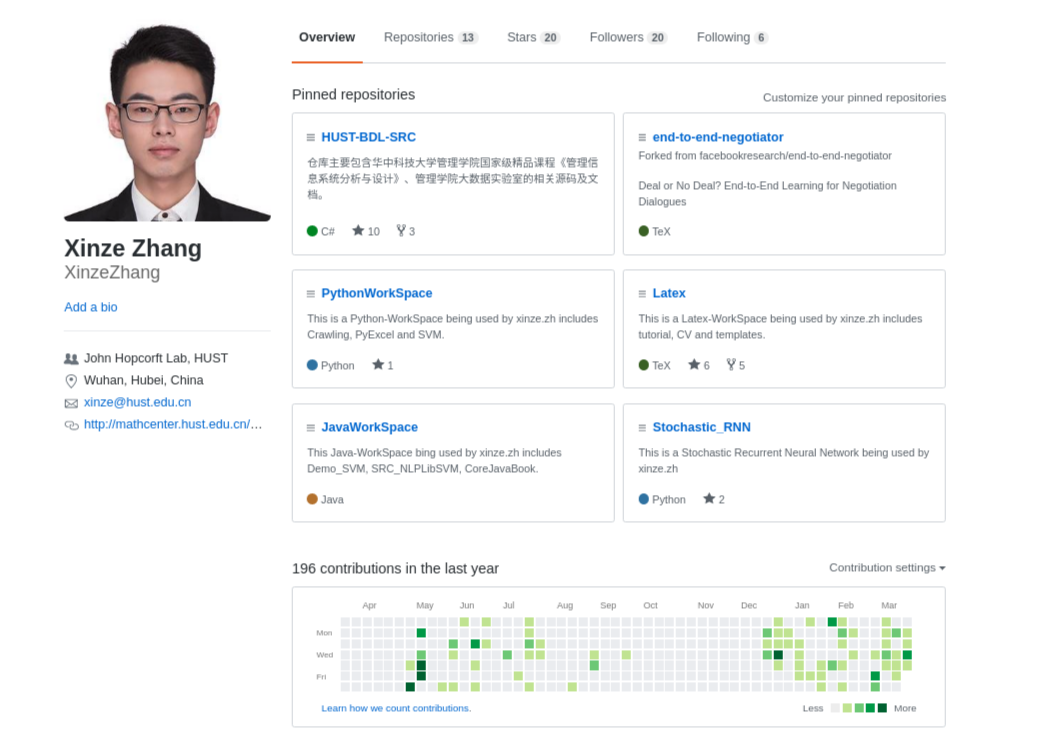
\includegraphics[width=\paperwidth]{./style/images/github.png}}
\begin{frame}[plain]

\end{frame}
}